\section{Support Class Reference}
\label{class_support}\index{Support@{Support}}
Class used to store additional informations in each node, here the support of the corresponding items.  


{\tt \#include $<$Support.hpp$>$}

Inheritance diagram for Support::\begin{figure}[H]
\begin{center}
\leavevmode
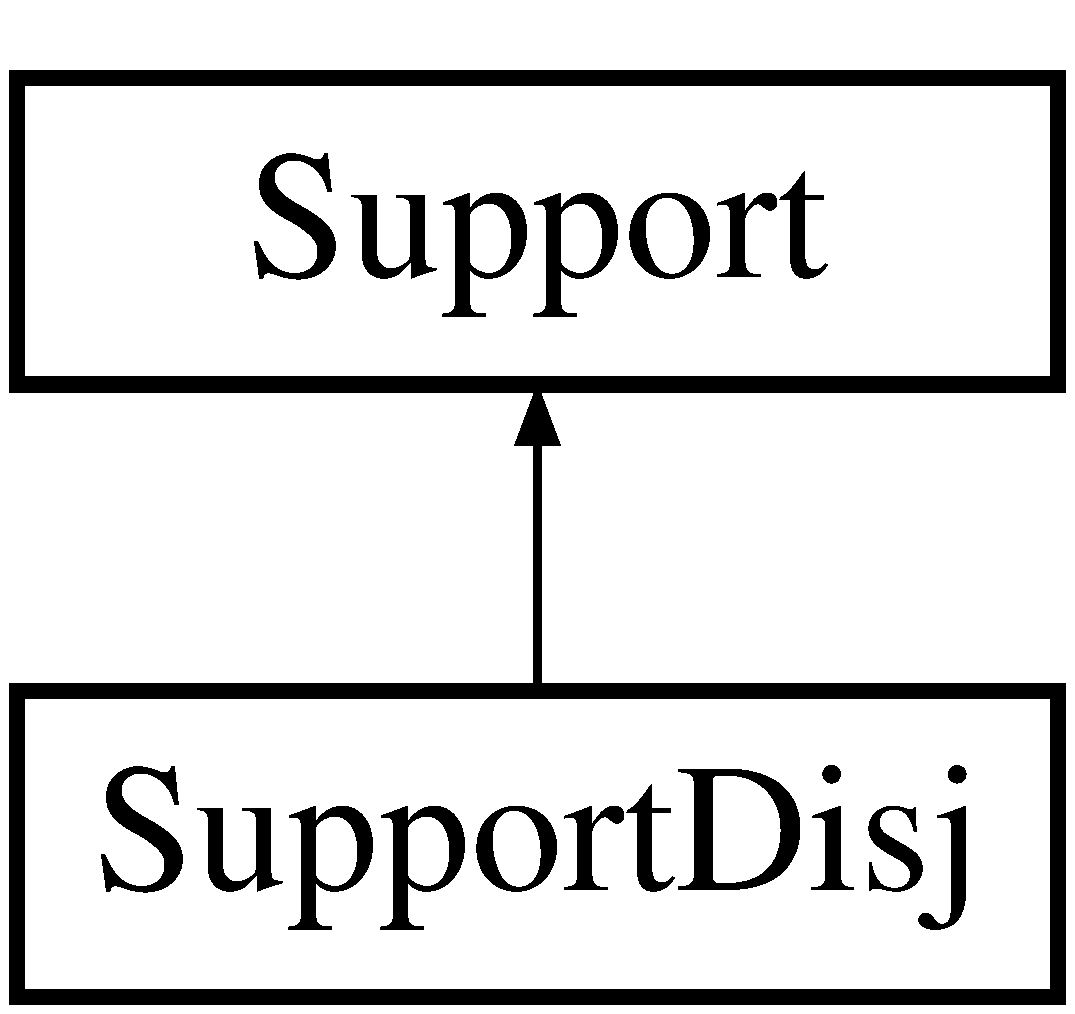
\includegraphics[height=2cm]{class_support}
\end{center}
\end{figure}
\subsection*{Public Member Functions}
\begin{CompactItemize}
\item 
{\bf Support} ()
\begin{CompactList}\small\item\em The constructor by deault, in cunjonction with the operator != to mark that an element is in a node. \item\end{CompactList}\end{CompactItemize}
\subsection*{Public Attributes}
\begin{CompactItemize}
\item 
bool {\bf presence}\label{class_support_1cb32d9c30dfd35099b9118e4234a5c2}

\begin{CompactList}\small\item\em used to not update the support of an itemset already considered \item\end{CompactList}\item 
int {\bf supp}\label{class_support_09e392dcc0f63feaa7b20513cfc8f630}

\begin{CompactList}\small\item\em store the support of the corresponding itemset \item\end{CompactList}\end{CompactItemize}


\subsection{Detailed Description}
Class used to store additional informations in each node, here the support of the corresponding items. 



\subsection{Constructor \& Destructor Documentation}
\index{Support@{Support}!Support@{Support}}
\index{Support@{Support}!Support@{Support}}
\subsubsection{\setlength{\rightskip}{0pt plus 5cm}Support::Support ()\hspace{0.3cm}{\tt  [inline]}}\label{class_support_19bf40018bf3004487c65f7e68c9f65e}


The constructor by deault, in cunjonction with the operator != to mark that an element is in a node. 

An element is in in the node is the {\bf Support}{\rm (p.\,\pageref{class_support})} of the current node is != of {\bf Support()}{\rm (p.\,\pageref{class_support_19bf40018bf3004487c65f7e68c9f65e})}. 

The documentation for this class was generated from the following file:\begin{CompactItemize}
\item 
F:/i\-Zi/problems/frequent/Support.hpp\end{CompactItemize}
